\documentclass[12pt]{article}
%\usepackage[utf8]{inputenc} %not needed for modern engines


% \usepackage{ragged2e}
% \justifying


% choose paragraph spacing and indentation
\setlength{\parskip}{12pt}   % vertical space between paragraphs
\setlength{\parindent}{0pt} % no paragraph indentation

\usepackage{amsmath}
\usepackage{amssymb}
\usepackage{geometry}
\usepackage{graphicx} %to import figures
\usepackage{subcaption} % provides \begin{subfigure}...\end{subfigure}
\usepackage{float}  %to place figures where you want
\usepackage{pgfplots} %to create graphs/figures natively
\pgfplotsset{compat=1.18} % set to the pgfplots version you have (or compat=newest)


\usepackage[italicdiff]{physics}
\usepackage[makeroom]{cancel}
\renewcommand{\familydefault}{\sfdefault}
\geometry{a4paper, margin=0.5in}

% --- add bibliography package ---
\usepackage{biblatex} %Imports biblatex package
\addbibresource{refs.bib} %Import the bibliography file



% --- user macros / shortcuts ---
% \providecommand{\vect}[1]{\ensuremath{\mathbf{#1}}}        % vector bold
\providecommand{\FT}[1]{\ensuremath{\mathcal{F}\{#1\}}}   % Fourier transform
\providecommand{\FTinverse}[1]{\ensuremath{\mathcal{F}^{-1}\{#1\}}}   % Fourier transform
% \providecommand{\norm}[1]{\ensuremath{\left\lVert#1\right\rVert}} % norm
\providecommand{\fresnelP}{\ensuremath{\frac{1}{i\lambda\Delta z}\,e^{\,i\frac{\pi}{\lambda\Delta z}(x^2+y^2)}}} % Fresnel kernel
\DeclareMathOperator{\sinc}{sinc} %?
\DeclareMathOperator{\sign}{sign}

% --- document info ---
\title{Holography\\Notes}
\author{By Nick Puentes}
\date{Winter 2025}



\begin{document}

\maketitle
\section{Holography}
Consider two plane waves that interfere.
Without loss of generality, we can have $A_0$ and $A_1$ be real since their phases are absorbed by $\phi(\mathbf{r})$.
\begin{align}
    I(\mathbf{r}) &= \qty(\hat{e}_{1}     A_1e^{i\vec{k}_{1}\cdot \mathbf{r}}e^{i \phi(\mathbf{r})} + 
    \hat{e}_{0}     A_0e^{i\vec{k}_{0}\cdot \mathbf{r}})
    \qty(\hat{e}_{1}    A_1e^{-i\vec{k}_{1}\cdot \mathbf{r}}e^{-i \phi(\mathbf{r})} + 
    \hat{e}_{0}     A_0e^{-i\vec{k}_{0}\cdot \mathbf{r}})\\
    &= |A_1|^2 + |A_0|^2 + 
    \hat{e}_{1}\cdot \hat{e}_{0}     A_1A_0\qty(e^{i(\vec{k}_1 - \vec{k}_0)\cdot \mathbf{r}}e^{i \phi(\mathbf{r})} + 
    e^{-i(\vec{k}_1 - \vec{k}_0)\cdot \mathbf{r}}e^{-i \phi(\mathbf{r})})\\
    &= |A_1|^2 + |A_0|^2 + \hat{e}_{1}\cdot \hat{e}_{0}     2A_1A_0 \cos((\vec{k}_1 - \vec{k}_0)\cdot \mathbf{r} + \phi(\mathbf{r}))
\end{align}
We can take the non-unitary, fourier transform of the intensity
\begin{align}
    \mathcal{F}[I(\mathbf{r})] &= (2\pi)^2 \delta^2(\mathbf{k})\qty(|A_1|^2 + |A_0|^2) + 
    \hat{e}_{1}\cdot \hat{e}_{0}     2A_1A_0 \mathcal{F}[\cos((\vec{k}_1 - \vec{k}_0)\cdot \mathbf{r} + \phi(\mathbf{r}))]
\end{align}

\begin{align}
    \mathcal{F}[\cos((\vec{k}_1 - \vec{k}_0)\cdot \mathbf{r} + \phi(\mathbf{r}))] 
    &= \frac{1}{2}\int d^2r 
        \qty(e^{(\vec{k}_1 - \vec{k}_0)\cdot \mathbf{r}} e^{i\phi(\mathbf{r})} + 
        e^{-(\vec{k}_1 - \vec{k}_0)\cdot \mathbf{r}} e^{-i\phi(\mathbf{r})}) 
        e^{-i\mathbf{k}\cdot \mathbf{r}}\\
    &= \frac{1}{2}
        \qty[\int d^2r e^{i\phi(\mathbf{r})}    e^{-i(\mathbf{k} - (\vec{k}_1 - \vec{k}_0))\cdot \mathbf{r}} + 
        \int d^2r e^{-i\phi(\mathbf{r})}     e^{-i(\mathbf{k} + (\vec{k}_1 - \vec{k}_0))\cdot \mathbf{r}} ]\\
    &= \frac{1}{2} \qty[
        \tilde{\Phi}_+ (\mathbf{k} - (\vec{k}_1 - \vec{k}_0)) + 
        \tilde{\Phi}_- (\mathbf{k} + (\vec{k}_1 - \vec{k}_0))]
\end{align}
Therefore, the fourier transform of the intensity is
\begin{equation}
    \mathcal{F}[I(\mathbf{r})] = (2\pi)^2 \delta^2(\mathbf{k})\qty(|A_1|^2 + |A_0|^2) + 
    \hat{e}_{1}\cdot \hat{e}_{0}     A_1A_0 
    \qty[\tilde{\Phi}_+ (\mathbf{k} - (\vec{k}_1 - \vec{k}_0)) + 
    \tilde{\Phi}_- (\mathbf{k} + (\vec{k}_1 - \vec{k}_0))]
\end{equation}
After capuring an image $I(\mathbf{r})$, numerically fourier transform the image and mask/select around 
the $+1$ mode, $\tilde{\Phi}_+ (\mathbf{k} - (\vec{k}_1 - \vec{k}_0))$. Note that both the image and its fourier transform 
will be affected by the point source function of the TEM, causing noise.

\section{Model Diffraction Gratings}
\subsection{Complex Index of Refraction}
The TEM chamber is nearly vacuum with an index of refraction taken as unity, 
and the speciem/object has some complex index of refraction $\tilde{n} = n + i\kappa$.
The real part changes the fields phase and the imaginary part\textemdash known as the 
extinction coefficient\textemdash attinuates the amplitude. The complex index of refraction 
is related to the complex wave number via
\begin{equation*}
    \boxed{\tilde{n} = \frac{c}{\omega} \tilde{k}}
\end{equation*}
A z-traveling plane wave in a vacuum is $e^{ik_z z}$. In some material with $\tilde{n}$, 
the plane wave is given by
\begin{align*}
    e^{i\tilde{k}_z z} &= e^{i(\frac{\omega}{c}(n + i\kappa)z)}\\
    &= e^{i(\frac{2\pi c}{\lambda c}(n + i\kappa)z)}\\
    &= e^{-\frac{2\pi \kappa}{\lambda}z}e^{i\frac{2\pi n}{\lambda}z}
\end{align*}
The wavelength, $\lambda$, is the vacuum wavelength.
\subsection{The Weak Phase Object}
\begin{equation}
    k_z = \frac{1}{\lambda} = \frac{\sqrt{eV(2m_0c^2 + eV)}}{hc}
\end{equation}



\section{Paraxial Helmholtz equation}
\begin{align*}
    \nabla_\perp^2 \psi(\mathbf{r}) + \frac{4\pi i}{\lambda} \pdv{\psi(\mathbf{r})}{z} = 0\\
    \pdv{\psi(\mathbf{r})}{z} = \frac{i\lambda}{4\pi} \nabla_\perp^2 \psi(\mathbf{r})
\end{align*}
which has the solution
\begin{equation*}
    \psi(x,y,z+\Delta z) = \exp(i \frac{\lambda \Delta z}{4\pi} \nabla_\perp^2) \psi(x,y,z)
\end{equation*}
Rewriting the paraxial Helmholtz equation in fourier space, using $\FT{\dv{x} f(x)} = i2\pi \xi \hat{f}(\xi)$ 
\begin{align*}
    -4\pi^2 (k_x^2 + k_y^2) \hat{\psi}(\mathbf{k}) + \frac{4\pi i}{\lambda} \pdv{\hat{\psi}(\mathbf{k})}{z} = 0\\
    \pdv{\hat{\psi}(\mathbf{k})}{z} = -i \pi \lambda (k_x^2 + k_y^2) \hat{\psi}(\mathbf{k})
\end{align*}

\section{fresnel propagation}

The fresnel propagation operator is given by Eq. 6.71 in 
\textit{Advanced Computing in Electron Microscopy} by Kirkland \cite{Kirkland2010}.
\begin{equation}\label{eq:fresnel_propagator}
    p(x,y, \Delta z) = \frac{1}{i\lambda \Delta z} e^{i \frac{\pi}{\lambda \Delta z} (x^2 + y^2)},
\end{equation}
The derivation of the fresnel propator required some notable considerations 
such as the paraxial approximation and requiring $(t \psi)$ were zero at infinity. There 
are plenty of other important considerations around this topic. The most important for 
my near future is that the order of operations matters for multislice simulations.


This convolution kernel is applied to the wavefunction as
\begin{equation*}
    \psi(x,y,z+\Delta z) = p(x,y,\Delta z)\ast \bigl[ t(x,y,z)\,\psi(x,y,z) \bigr]
\end{equation*}
where $t(x,y,z)$ is the transmission function at slice $z$.
\subsection{w/ converging lens}
A field in the back focal plane, $\psi_0$, of a converging thin lens with focal length $F$ transforms into $\psi_{2F}$ 
in the front focal plane according to
 \begin{equation}
    \psi_{2F}(x,y) = \frac{e^{i2kF}}{i\lambda F} \hat{\psi_0}\qty(\frac{x}{\lambda F}, \frac{y}{\lambda F})
\end{equation}


\begin{figure}[H]
    \centering
    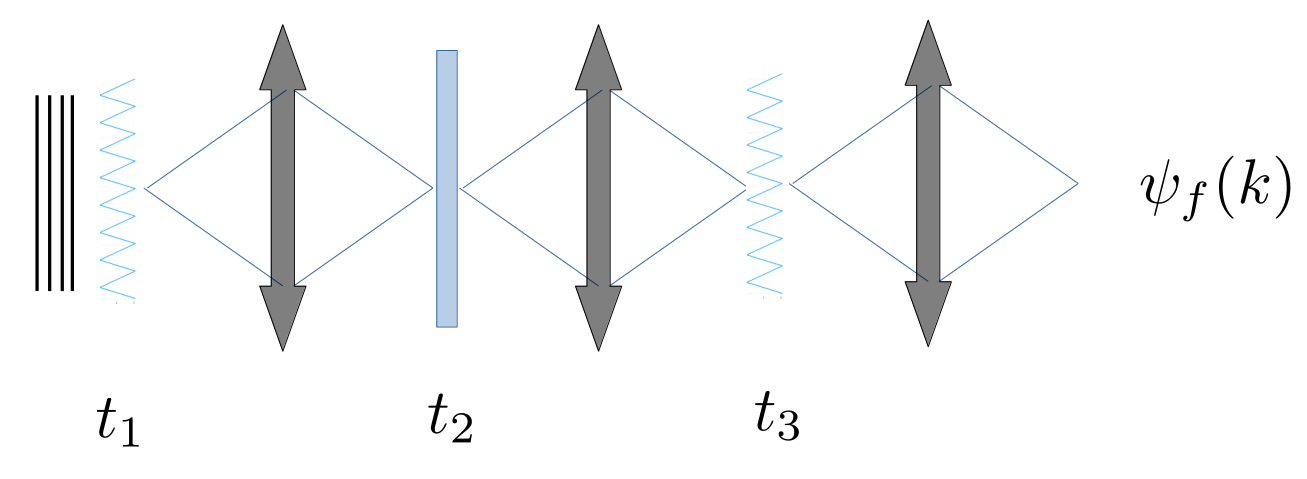
\includegraphics[width=0.8\textwidth]{figures/IFM_setup.png}
    \caption{Interferometric setup for the IFM experiment.}
    \label{fig:IFM_setup}
\end{figure}
The wavefunction at the detector plane is given by
\begin{align}
    \psi_{4}^{-} &= \frac{e^{i2kF_3}}{i\lambda F_3} \FT{
                    t_3 \frac{e^{i2kF_2}}{i\lambda F_2} \FT{
                        t_2 \frac{e^{i2kF_1}}{i\lambda F_1} \FT{
                            t_1 \psi_0}}}\\
    &= \frac{e^{i2kF_3}}{i\lambda F_3} 
    \frac{e^{i2kF_2}}{i\lambda F_2}
    \frac{e^{i2kF_1}}{i\lambda F_1}
    \FT{t_3 \FT{t_2 \FT{t_1 \psi_0}}}\\
    &\propto
    \FT{t_3 \FT{t_2 \hat{t_1}}} \, \qq{w/ $\psi_0$ as a plane wave}\\
\end{align}
using the convolution theorem and two forward fourier transforms
\begin{align*}
    \FT{\FT{r(x)}} = r(-x)\\
    \{u \ast v \}(-f) = \FT{U \cdot V}
\end{align*}
\begin{align*}
    \FT{t_3 \FT{t_2 \hat{t_1}}} &= \{\FTinverse{t_3} \ast \qty(t_2 \hat{t_1})\}(-f)\\
    &= \{ \mathcal{P} \hat{t_3} \ast (t_2 \hat{t_1})\}(-f)\\
    &= \int d\xi \, \hat{t_3}(-(-f - \xi)) t_2(\xi) \hat{t_1}(\xi)\\
    &= \int d\xi \, \hat{t_3}(\xi + f) t_2(\xi) \hat{t_1}(\xi)
\end{align*}
The connection between the Fourier Transform and the Fourier coefficients can be seen with
the Fourier Transform of a periodic function with period p:
\begin{equation*}
    \FT{t_i(x)}(\xi) = \sum_{-\infty}^{\infty} c^{\{i\}}_n \cdot \delta(\xi - \frac{n}{p_i})
\end{equation*}
\begin{align*}
    \FT{t_3 \FT{t_2 \hat{t_1}}} &= 
    \int d\xi \, \hat{t_3}(\xi + f) t_2(\xi) \hat{t_1}(\xi)\\
    &= \int d\xi \,\qty(\sum_{m=-\infty}^{\infty} c^{\{3\}}_m \delta(\xi + f - \frac{m}{p_3}))
        t_2(\xi)
        \qty(\sum_{n=-\infty}^{\infty} c^{\{1\}}_n \delta(\xi - \frac{n}{p_1}))\\
    &= \sum_{m,n=-\infty}^{\infty} \int d\xi \, c^{\{3\}}_m 
        \delta(\xi + f - \frac{m}{p_3}) \,
        t_2(\xi) \,
        c^{\{1\}}_n \delta(\xi - \frac{n}{p_1})\\
    &= \sum_{m,n=-\infty}^{\infty} \, c^{\{3\}}_m 
        \delta_{\frac{n}{p_1}}^{\frac{m}{p_3}-f} \,
        t_2\qty(\frac{n}{p_1}) \,
        c^{\{1\}}_n \\
    &= \sum_{m,n=-\infty}^{\infty} \, c^{\{3\}}_m 
        \delta_{\frac{p_3}{p_1}n+p_3 f}^{m} \,
        t_2\qty(\frac{n}{p_1}) \,
        c^{\{1\}}_n \\
\end{align*}
$m = \frac{p_3}{p_1}n+p_3 f = \frac{p_3}{p_1}n+p_3 (\Delta f) \ell$, implying $\frac{p_3}{p_1} \in \mathbb{Z}$ and $\Delta f = \frac{1}{p_3}$.
\begin{equation}
    \boxed{
    \psi\qty(\frac{\ell}{p_3}) = 
    \sum_{n=-\infty}^{\infty} \,
     c^{\{3\}}_{\frac{p_3}{p_1}n + \ell} \,
        t_2\qty(\frac{n}{p_1}) \,
        c^{\{1\}}_n 
    }
\end{equation}
From here after, we are setting $p_1 = p_3 = 1$ for simplicity. Moreover, let's suppose that 
$t_2$ can be written with the same functional form as $t_1$ and $t_3$: 
$t_2(x) = \exp{i \kappa^{\{2\}} d^{\{2\}}(x)}$. Therefore, the wavefunction at the image plane is
\begin{equation*}
    \psi_\ell = 
    \sum_{n=-\infty}^{\infty} \,
     c^{\{3\}}_{n + \ell} \,
        \exp{i \kappa^{\{2\}} d^{\{2\}}_n} \,
        c^{\{1\}}_n 
\end{equation*}


\section{Fisher Information}
\subsection{definition}
The fisher information matrix for a set of parameters $\theta = \left[\theta_1, \theta_2, \dots, \theta_n\right]$ is defined as
\begin{equation*}
    \qty[I(\theta)]_{m,w} = 
    \mathbb{E}\qty[
        \qty(\pdv{\theta_m} \ln(f(x\mid \theta)))
        \qty(\pdv{\theta_w} \ln(f(x\mid \theta)))
        ]
\end{equation*}
where $f(x\mid \theta)$ is the probability density function of the data $x$ given the parameters $\theta$.

\subsection{Poissonian Statistics}
Since electron emission is goverened by poissonian statistics, the electron count
probability at the detector is given by $f(k\mid \lambda) = \frac{\lambda^k e^{-\lambda}}{k!}$, 
where $\lambda = |\psi_\ell|^2$. Note that $\lambda$ is implicitly a function of $\ell$, i.e. the 
particular mode under consideration. To acquire the total fisher information matrix that includes 
all modes, requires summing over all modes (e.g. $I(\theta) = \sum_{\ell} I_\ell (\theta)$).
\begin{align*}
    \pdv{\lambda} \ln(f(k\mid \lambda)) &= \pdv{\lambda} \qty( k \ln(\lambda) - \lambda - \ln(k!)) = \frac{k}{\lambda} - 1 = \frac{k-\lambda}{\lambda}\\
    I(\lambda) &= \mathbb{E}\qty[\qty(\pdv{\lambda} \ln(f(k\mid \lambda)))^2] \\
    &= \mathbb{E}\qty[\qty(\frac{k-\lambda}{\lambda})^2] \\
    &= \frac{1}{\lambda^2} \mathrm{Var}(k) = \frac{1}{\lambda^2} \lambda = \frac{1}{\lambda}
\end{align*}

Suppose that $\lambda$ is a function of the parameters $\theta$, then the fisher information matrix elements are
\begin{align*}
    \qty[I(\theta)]_{m,w} &= 
    \mathbb{E}\qty[
        \qty(\pdv{\theta_m} \ln(f(k\mid \lambda)))
        \qty(\pdv{\theta_w} \ln(f(k\mid \lambda)))
        ] \\
    &= \mathbb{E}\qty[
        \qty(\pdv{\lambda} \ln(f(k\mid \lambda)))^2 
        ] \pdv{\theta_m} \lambda \pdv{\theta_w} \lambda  \\
    &= \frac{1}{\lambda} \pdv{\theta_m} \lambda \pdv{\theta_w} \lambda
\end{align*}

More generally for a particular mode $\ell$,
\begin{equation*}
    \boxed{
    I_\ell(\theta) = 
    \frac{1}{\lambda_\ell} \nabla \lambda_\ell \nabla^T \lambda_\ell
    }
\end{equation*}
and for all modes $\ell$
\begin{equation*}
    \boxed{
    I(\theta) = \sum_{\ell}
    \frac{1}{\lambda_\ell} \nabla \lambda_\ell \nabla^T \lambda_\ell
    }
\end{equation*}
where $\nabla \lambda_\ell = \begin{bmatrix}
    \pdv{\theta_1}  \\
    \pdv{\theta_2} \\
    \vdots \\
    \pdv{\theta_n} 
\end{bmatrix} \lambda_\ell$.

\subsection{Background Noise}
Detectors have background poissonian noise that can be included with 
\begin{equation*}
        \lambda_{\ell, \text{noisy}} = N \qty(|\psi_\ell|^2 + \frac{b_\ell}{N})
\end{equation*}
where $N$ is the total number of electrons that enter the sample plane. Side note: 
the interpretation of $N$ can change depending on how $\psi$ is normalized. For 
instance, if $\psi$ is normalized just before the first grating (G1), then $N$ is the total 
number of electrons interacting with G1. We want to know the number of electrons that are in 
the sample plain to properly account for sample damage, which can be done by normalizing $\psi$ 
after G1 and before the sample. $b_\ell$ is the background noise counts at mode $\ell$. For this case,
the noise for each mode, $b_\ell$ , should be independent of model parameters and mode, but we 
will keep the $\ell$ supscript to remind us of its role.

Let's have $\lambda_\ell = |\psi_\ell|^2$, so the FIM is
\begin{align*}
    I(\theta) &= \sum_{\ell}
    \frac{1}{\lambda_{\ell, \text{noisy}}} \nabla \lambda_{\ell, \text{noisy}} \nabla_\theta^T \lambda_{\ell, \text{noisy}}\\
    &= N\sum_{\ell} \frac{1}{\lambda_\ell + \frac{b_\ell}{N}} \nabla \lambda_\ell \nabla_\theta^T \lambda_\ell\\
    &= N\sum_{\ell} \frac{1}{\lambda_\ell} \nabla \lambda_\ell \nabla^T \lambda_\ell 
        \qty(1 + \frac{b_\ell}{\lambda_\ell N})^{-1}\\
\end{align*}
\begin{equation*}
    \boxed{
    I(\theta) = N\sum_{\ell} 
    \frac{1}{\lambda_\ell} \nabla \lambda_\ell \nabla^T \lambda_\ell 
        \qty(1 + \frac{b_\ell}{\lambda_\ell N})^{-1}
    }
\end{equation*}
We retrieve the noiseless FIM, but now each mode is attenuated by the 
monotonically decreasing factor $\qty(1 + \frac{b_\ell}{\lambda_\ell N})^{-1}$, 
which has domain $[0,\infty)$ and range (0,1].

\textbf{comments} The inclusion of background noise is important for simulations/calculations because the 
attenuating factor significantly reduces the contribution of modes with low counts ($|\psi_\ell|^2<<1$). 
To elaborate, consider the case where we had a noiseless detector and a mode with $|\psi_\ell|^2=\epsilon$, 
or $|\psi_\ell|^2<<1$, then detecting an electron at that mode is extremely informative. However, background 
noise makes these informative detections imposible to identify.

    

\subsection{standard basis}
\begin{equation*}
    \psi_\ell = 
    \sum_{n=-\infty}^{\infty} \,
     c^{\{3\}}_{n + \ell} \,
        \exp{i \kappa^{\{2\}} d^{\{2\}}_n} \,
        c^{\{1\}}_n 
\end{equation*}
The fisher information matrix elements for parameters $d^{\{2\}}_m$ and $d^{\{2\}}_w$ are given by
\begin{align*}
    \qty[I(d^{\{2\}})]_{m,w} &= 
    \mathbb{E}\qty[
        \qty(\pdv{d^{\{2\}}_m} \ln(f(k\mid \lambda)))
        \qty(\pdv{d^{\{2\}}_w} \ln(f(k\mid \lambda)))
        ] \\
    &= \mathbb{E}\qty[
        \qty(\pdv{\lambda} \ln(f(k\mid \lambda)))^2 
        ] \pdv{d^{\{2\}}_m} \lambda \pdv{d^{\{2\}}_w} \lambda  \\
    &= \frac{1}{\lambda} \pdv{d^{\{2\}}_m} \lambda \pdv{d^{\{2\}}_w} \lambda \\
    &= \frac{4}{\lambda} \Re\qty(\psi_\ell^* \pdv{d^{\{2\}}_m} \psi_\ell)
        \Re\qty(\psi_\ell^* \pdv{d^{\{2\}}_w} \psi_\ell)
\end{align*}

\begin{align*}
    \pdv{d^{\{2\}}_m} \lambda &= \pdv{d^{\{2\}}_m} |\psi_\ell|^2 = \psi_\ell^* \pdv{d^{\{2\}}_m} \psi_\ell + \psi_\ell \pdv{d^{\{2\}}_m} \psi_\ell^* \\
    \pdv{d^{\{2\}}_m} \psi_\ell &= 
    \sum_{j=-\infty}^{\infty} 
        c^{\{3\}}_{j + \ell} 
        \qty(i \kappa^{\{2\}} \delta_{j,m} e^{i \kappa^{\{2\}} d^{\{2\}}_j}) 
        c^{\{1\}}_j\\
    &= i \kappa^{\{2\}} 
        c^{\{3\}}_{m + \ell} 
        e^{i \kappa^{\{2\}} d^{\{2\}}_m} 
        c^{\{1\}}_m
\end{align*}


\begin{align*}
    2\Re\qty(\psi_\ell^* \pdv{d^{\{2\}}_m} \psi_\ell) &= 
    \qty(\sum_{j=-\infty}^{\infty} 
        c^{\{3\}*}_{j + \ell} 
        e^{-i \kappa^{\{2\}} d^{\{2\}}_j} 
        c^{\{1\}*}_j 
    )\cdot
        i \kappa^{\{2\}} 
        c^{\{3\}}_{m + \ell} 
        e^{i \kappa^{\{2\}} d^{\{2\}}_m} 
        c^{\{1\}}_m + c.c.\\
    \frac{1}{|\psi|}\qty(\psi_\ell^* \pdv{d^{\{2\}}_m} \psi_\ell + c.c.) &= 
    e^{-i \arg{\psi_\ell}}\pdv{d^{\{2\}}_m} \psi_\ell + c.c\\
    &= e^{-i \arg{\psi_\ell}} i \kappa^{\{2\}} 
        c^{\{3\}}_{m + \ell} 
        e^{i \kappa^{\{2\}} d^{\{2\}}_m} 
        c^{\{1\}}_m + c.c.\\
    &=-2 |\kappa^{\{2\}}| 
        |c^{\{3\}}_{m + \ell}|
        e^{-\kappa_i^{\{2\}} d^{\{2\}}_m}  
        |c^{\{1\}}_m|\\
        &\cdot \sin\qty(
            - \arg{\psi_\ell} 
            + \arg{\kappa^{\{2\}}}
            + \arg{c^{\{3\}}_{m + \ell}}
            + \kappa_r^{\{2\}} d^{\{2\}}_m 
            + \arg{c^{\{1\}}_m}
            )
\end{align*}
\begin{align*}
    \qty[I(d^{\{2\}})]_{m,w} &= 
    4 |\kappa^{\{2\}}|^2 
    |c^{\{3\}}_{m + \ell}|
    |c^{\{1\}}_m| \,
    |c^{\{3\}}_{w + \ell}|
    |c^{\{1\}}_w| e^{-\kappa_i^{\{2\}} (d^{\{2\}}_w+d^{\{2\}}_m)}   \\
    &\cdot \sin\qty(
        - \arg{\psi_\ell} 
        + \arg{\kappa^{\{2\}}}
        + \arg{c^{\{3\}}_{m + \ell}}
        + \kappa_r^{\{2\}} d^{\{2\}}_m 
        + \arg{c^{\{1\}}_m}
        )\\
    &\cdot \sin\qty(
        - \arg{\psi_\ell} 
        + \arg{\kappa^{\{2\}}}
        + \arg{c^{\{3\}}_{w + \ell}}
        + \kappa_r^{\{2\}} d^{\{2\}}_w 
        + \arg{c^{\{1\}}_w}
        )
\end{align*}



\subsection{fisher information in rotated basis}
Let consider only two beams hitting the sample, $c^{\{ 1 \}}_{0}$ and $c^{\{ 1 \}}_1$. 
Let $\Delta d = d^{\{ 2 \}}_1 - d^{\{ 2 \}}_0$ and 
$\Sigma d = d^{\{ 2 \}}_1 + d^{\{ 2 \}}_0$. The wavefunction at the image plane is
\begin{align*}
    \psi_\ell &= 
     c^{\{3\}}_{0 + \ell} \,
        \exp{i \kappa^{\{2\}} d^{\{2\}}_0} \,
        c^{\{1\}}_0 +
     c^{\{3\}}_{1 + \ell} \,
        \exp{i \kappa^{\{2\}} d^{\{2\}}_1} \,
        c^{\{1\}}_1 \\
    &= 
     c^{\{3\}}_{\ell} \,
        \exp{i \kappa^{\{2\}} \frac{\Sigma d - \Delta d}{2}} \,
        c^{\{1\}}_0 +
     c^{\{3\}}_{1 + \ell} \,
        \exp{i \kappa^{\{2\}} \frac{\Sigma d + \Delta d}{2}} \,
        c^{\{1\}}_1
\end{align*}
\begin{align*}
    \pdv{\psi_\ell}{\Delta d} &= 
        \pdv{\Delta d}\left( \alpha_\ell + \beta_\ell \right) 
        = \qty(\frac{i\kappa}{2})(-\alpha_\ell + \beta_\ell) \\
    \pdv{\psi_\ell}{\Sigma d} &= 
        \pdv{\Sigma d}\left( \alpha_\ell + \beta_\ell \right) 
        = \qty(\frac{i\kappa}{2})(\alpha_\ell + \beta_\ell)
        = \frac{i\kappa}{2} \psi_\ell
\end{align*}
\begin{align*}
    \frac{1}{|\psi_\ell|} \pdv{\Sigma d} |\psi_\ell|^2 &= 
    \frac{1}{|\psi_\ell|} \qty(\psi_\ell^* \pdv{\Sigma d} \psi_\ell + c.c.) 
    = \qty(\frac{i\kappa}{2})\psi_\ell e^{-i \arg{\psi_\ell}} + c.c. 
    = -\kappa_i |\psi_\ell| \\
    \frac{1}{|\psi_\ell|} \pdv{\Delta d} |\psi_\ell|^2 &=
    \frac{1}{|\psi_\ell|} \qty(\psi_\ell^* \pdv{\Delta d} \psi_\ell + c.c.) \\
        &= \qty(\frac{i\kappa}{2})(-\alpha_\ell + \beta_\ell)e^{-i \arg{\psi_\ell}} + c.c. \\
        &= \qty(\frac{i\kappa}{2})(\psi_\ell-2\alpha_\ell)e^{-i \arg{\psi_\ell}} + c.c. \\
        &= -\kappa_i |\psi_\ell| + 
            2 \Re{ \qty(\frac{i\kappa}{2})(-2\alpha_\ell)e^{-i \arg{\psi_\ell}}}\\
        &= -\kappa_i |\psi_\ell| + 2 |\kappa| 
            |\alpha_\ell| \sin(\arg{\kappa} + \arg{\alpha_\ell} - \arg{\psi_\ell})
\end{align*}

The FIM can be constructed in this rotated basis by taking an outer product using the 
two above expressions. This can be found, with an error (extra minus sign), in 
\texttt{Notebook\_202511\_202601} Pg~51--52. 
We are more interested in constructing the FIM in a more symmetric way, treating both terms 
$\alpha$ and $\beta$ equally (as opposed to singling out $\alpha$ like above).

Starting from the above derivatives 
\begin{align*}
    \pdv{\Sigma d} |\psi_\ell|^2 &= 
    \qty(\psi_\ell^* \pdv{\Sigma d} \psi_\ell + c.c.) 
    = \psi_\ell^*\qty(\frac{i\kappa}{2})\psi_\ell  + c.c. 
    = -\kappa_i |\psi_\ell|^2 \\
    \pdv{\Delta d} |\psi_\ell|^2 &=
    \qty(\psi_\ell^* \pdv{\Delta d} \psi_\ell + c.c.) \\
        &= \qty(\frac{i\kappa}{2})(-\alpha_\ell + \beta_\ell)(\alpha_\ell^* + \beta_\ell^*) + c.c. \\
        &= \qty(\frac{i\kappa}{2})
            \qty( 
                (|\beta_\ell|^2 - |\alpha_\ell|^2)  + 
                (\beta_\ell \alpha_\ell^* - \alpha_\ell \beta_\ell^*)
            ) + c.c. \\
        &= \qty(\frac{i\kappa}{2})
            \qty( 
                (|\beta_\ell|^2 - |\alpha_\ell|^2)  + 
                2i\Im{\alpha_\ell^*\beta_\ell}
            ) + c.c.\\
        &= -\kappa_i (|\beta_\ell|^2 - |\alpha_\ell|^2) - 
            \kappa_r 2 \Im{\alpha_\ell^*\beta_\ell}
\end{align*}
where $\Im{\alpha_\ell^*\beta_\ell} = |\alpha_\ell||\beta_\ell|\sin(\delta_\ell)$ 
with $\delta_\ell \equiv \arg{\beta_\ell} - \arg{\alpha_\ell} 
= \kappa_r (d_1 - d_0) + \arg(c_{1+\ell} c_{1}) - \arg(c_{0+\ell} c_{0})$.
The noiseless 2 by 2 fisher information matrix in this rotated basis is 
\begin{align*}
    I_\ell &= 
    \frac{1}{\lambda_\ell} \begin{bmatrix}
    \pdv{\Delta d} \lambda_\ell \\
    \pdv{\Sigma d} \lambda_\ell\\
\end{bmatrix}
\begin{bmatrix}
    \pdv{\Delta d} \lambda_\ell &
    \pdv{\Sigma d} \lambda_\ell \\
\end{bmatrix}\\
&=
\frac{1}{|\psi_\ell|^2} \begin{bmatrix}
    \qty(\kappa_i (|\beta_\ell|^2 - |\alpha_\ell|^2) + 
        \kappa_r 2 \Im{\alpha_\ell^*\beta_\ell})^2 &
    \qty(\kappa_i (|\beta_\ell|^2 - |\alpha_\ell|^2) + 
        \kappa_r 2 \Im{\alpha_\ell^*\beta_\ell})(\kappa_i |\psi_\ell|^2) \\
    \qty(\kappa_i |\psi_\ell|^2)
    \qty(\kappa_i (|\beta_\ell|^2 - |\alpha_\ell|^2) + 
        \kappa_r 2 \Im{\alpha_\ell^*\beta_\ell}) &
    \qty(\kappa_i |\psi_\ell|^2)^2 
\end{bmatrix} 
\end{align*}
The FIM can be rewritten in terms of $S_\ell = |\alpha_\ell|^2+|\beta_\ell|^2$, 
$s_\ell =\sign(|\beta_\ell|^2 - |\alpha_\ell|^2)$, and 
$V_\ell = \frac{2|\alpha_\ell||\beta_\ell|}{|\alpha_\ell|^2+|\beta_\ell|^2}$ :
\begin{align*}
    I_\ell &= \frac{u_\ell u_\ell^T}{S_\ell (1+V_\ell \cos(\delta_\ell))}, \\
    u_\ell &= -S_\ell \begin{bmatrix}
        \kappa_i s_\ell\sqrt{1-V_\ell^2} + \kappa_r V_\ell \sin(\delta_\ell) \\
        \kappa_i (1+V_\ell \cos(\delta_\ell))
    \end{bmatrix}
\end{align*}
or with noise $I_\ell = (S_\ell (1+V_\ell \cos(\delta_\ell)) + \frac{b_\ell}{N})^{-1} u_\ell u_\ell^T$.
Let $\kappa_i = 0$ for the noiseless case
\begin{align*}
    I_\ell &= \frac{\kappa_r^2 S_\ell V_\ell^2 \sin^2(\delta_\ell)}{1+V_\ell \cos(\delta_\ell)}
    \begin{bmatrix}
        1 & 0 \\
        0 & 0
    \end{bmatrix}
\end{align*}


\subsection{standard basis}
Let there be two beams, where only one hits the sample.
\begin{align*}
    \psi_\ell &= 
    c^{\{3\}}_{0 + \ell} \, 
    c^{\{1\}}_0 
    + c^{\{3\}}_{1 + \ell} \,
        \exp{i \kappa^{\{2\}} d^{\{2\}}_1} \,
        c^{\{1\}}_1 \\
        &= \alpha_\ell + \beta_\ell\\
    |\psi_\ell|^2 &= |\alpha_\ell|^2 + |\beta_\ell|^2 + 2\Re{\alpha_\ell^* \beta_\ell}\\
    &= |\alpha_\ell|^2 + |\beta_\ell|^2 + 2|\alpha_\ell||\beta_\ell|\cos(\delta_\ell)
\end{align*}
where $\delta_\ell = \kappa_r d^{\{2\}}_1 + \arg(c_{1+\ell} c_{1}) - \arg(c_{0+\ell} c_{0})$.

\begin{align*}
    \pdv{d^{\{2\}}_1} |\psi_\ell|^2 &= 
    -2\kappa_i |\beta_\ell|^2 
    - 2\kappa_i|\alpha_\ell||\beta_\ell|\cos(\delta_\ell) 
    - 2\kappa_r |\alpha_\ell||\beta_\ell|\sin(\delta_\ell)\\
    &= -2\kappa_i(|\alpha_\ell||\beta_\ell|\cos(\delta_\ell) + |\beta_\ell|^2) 
    - 2\kappa_r |\alpha_\ell||\beta_\ell|\sin(\delta_\ell)\\
    &= -2|\alpha_\ell||\beta_\ell|\kappa_r \left(
        \sin(\delta_\ell) + \frac{\kappa_i}{\kappa_r} \left(\cos(\delta_\ell) + \frac{|\beta_\ell|}{|\alpha_\ell|}\right)  
    \right)
\end{align*}
\begin{align*}
    \left( \pdv{d^{\{2\}}_1} |\psi_\ell|^2 \right)^2 &=
    4|\alpha_\ell|^2|\beta_\ell|^2\kappa_r^2 \left(
        \sin(\delta_\ell) + \frac{\kappa_i}{\kappa_r} \left(\cos(\delta_\ell) + \frac{|\beta_\ell|}{|\alpha_\ell|}\right)  
    \right)^2   
\end{align*}

\begin{align*}
    I_\ell &= \frac{1}{\lambda_\ell} \qty(\pdv{d^{\{2\}}_1} |\psi_\ell|^2)^2 \\
    &= \frac{4|\alpha_\ell|^2|\beta_\ell|^2\kappa_r^2}{|\psi_\ell|^2} 
    \left(
        \sin(\delta_\ell) + \frac{\kappa_i}{\kappa_r} \left(\cos(\delta_\ell) + \frac{|\beta_\ell|}{|\alpha_\ell|}\right)  
    \right)^2\\
    &= \frac{4|\alpha_\ell|^2|\beta_\ell|^2\kappa_r^2}{|\alpha_\ell|^2 + |\beta_\ell|^2 + 2|\alpha_\ell||\beta_\ell|\cos(\delta_\ell)} \left(
        \sin(\delta_\ell) + \frac{\kappa_i}{\kappa_r} 
        \left(\cos(\delta_\ell) + \frac{|\beta_\ell|}{|\alpha_\ell|}\right) 
    \right)^2\\
    &= \frac{\kappa_r^2 V_\ell^2 S_\ell}{ 1 + V_\ell \cos(\delta_\ell)}
     \left(
        \sin(\delta_\ell) + \frac{\kappa_i}{\kappa_r} 
        \left(\cos(\delta_\ell) + \frac{|\beta_\ell|}{|\alpha_\ell|}\right) 
    \right)^2
\end{align*}
where $S_\ell = |\alpha_\ell|^2 + |\beta_\ell|^2$ and $V_\ell = \frac{2|\alpha_\ell||\beta_\ell|}{|\alpha_\ell|^2 + |\beta_\ell|^2}$.


\subsection{2 by 2 fisher information matrix}
given 
\begin{align*}
    \frac{1}{\sqrt{\lambda_\ell}} \pdv{d^{\{2\}}_m} \lambda_\ell &=
    \frac{1}{|\psi|}\qty(\psi_\ell^* \pdv{d^{\{2\}}_m} \psi_\ell + c.c.) \\ 
        &=-2 |\kappa^{\{2\}}| 
            |c^{\{3\}}_{m + \ell}|
            e^{-\kappa_i^{\{2\}} d^{\{2\}}_m}  
            |c^{\{1\}}_m|\\
            &\cdot \sin\qty(
                - \arg{\psi_\ell} 
                + \arg{\kappa^{\{2\}}}
                + \arg{c^{\{3\}}_{m + \ell}}
                + \kappa_r^{\{2\}} d^{\{2\}}_m 
                + \arg{c^{\{1\}}_m}
                )
\end{align*}
let's create a vector $u_\ell$ with components of $m=0$ and $m=1$
\begin{equation*}
    u_\ell = \frac{1}{\sqrt{\lambda_\ell}} \begin{bmatrix}
        \pdv{d^{\{2\}}_0}  \\
        \pdv{d^{\{2\}}_1} 
    \end{bmatrix} \lambda_\ell
\end{equation*}

The 2 by 2 Fisher information matrix is then
\begin{equation*}
    I = \sum_\ell u_\ell u_\ell^T
\end{equation*}

\section{two-grating misalignment}
One large issue in performing the 2GMZI experiment is the misalignment of the two gratings. 
Assuming that the two gratings are in the same dual plane, the first grating (G1) projects 
its image onto the second grating (G2), which induces lateral, rotational, and magnification 
offsets. The lateral offset is the most benign of these three because G2 can be laterally shifted 
to alignment and the lateral offset of the gratings does not distort the diffraction spots\textemdash
only the lateral offset between the circular apertures distorts the diffraction spots. The 
magnification and rotational offsets are analyzed by considering the convolution between their 
fourier coefficients.  

using the law of cosines
\begin{align*}
    \cos(\theta) &= \frac{L_2^2 + L_1^2 - R^2}{2L_1L_2}
\end{align*}
defining $M = \frac{L_2}{L_1}$
\begin{align*}
    \cos(\theta) &= \frac{L_1^2 + L_1^2 M^2 - R^2}{2M L_1^2} = \frac{1 + M^2 - R^2/L_1^2}{2M}\\
    &=\frac{1 + M^2 - R^2 M^2/L_2^2}{2M}
\end{align*}
Set $R = \frac{r_{\text{airy}}}{2}$ and let $\rho = \frac{r_{\text{airy}}}{r_{\text{sep}}}$, 
where $r_{\text{sep}} = 2L_2$ is the separation between G2's diffraction spots 
and $r_{\text{airy}}$ is the radius of the airy point spread function. 
\begin{align*}
    \boxed{\cos(\theta) = \frac{1 + M^2\qty(1 - \rho^2)  }{2M}}  
\end{align*}
This equation relates the maximum rotational misalignment $\theta$ to the magnification $M$ of G1
onto G2 ($M=\frac{L_2}{L_1} = \frac{p_1}{p_2}$ diffraction space length and real space pitch) and 
the ratio $\rho$ of the airy disk radius to the separation between diffraction spots. Detailed 
algebra can be found in \texttt{Notebook\_202602\_2026xx} Pg~38--42. 

Lets consider the case where $M=1$, 
\begin{align*}
    \cos(\theta) &= 1 - \frac{\rho^2}{2} \\
    \theta &\approx \rho \quad \text{for small $\rho$}
\end{align*}

In looking at this equation, the magnification $M$ and $\rho$ are bounded by the domain 
of $\cos(\theta)$. Setting cosine to unity gives solutions for $M$ given $\rho$: 
\begin{align*}
    M = \frac{1}{1\pm \rho}
\end{align*}
There are physical/practical constraints on $\rho = \frac{r_{\text{airy}}}{r_{\text{sep}}} = \frac{R}{L_2}$. 
I chose a conservative value of $\rho = \frac{1}{3}$ to ensure that the diffraction modes don't leak into 
other modes. This value was chosen by considering $\theta=0$ and that there should be a distance of $R$ before 
touching the next diffraction spot, which gives $R = \frac{r_{\text{sep}}}{3}$ or $r_{\text{sep}} = 3R$. This value 
should prevent leakage. However, it may be worth exploring $r_{\text{sep}} = 2R$ since the center of the 
diffraction spot still has low leakage. 

\begin{figure}[H]
    \centering
    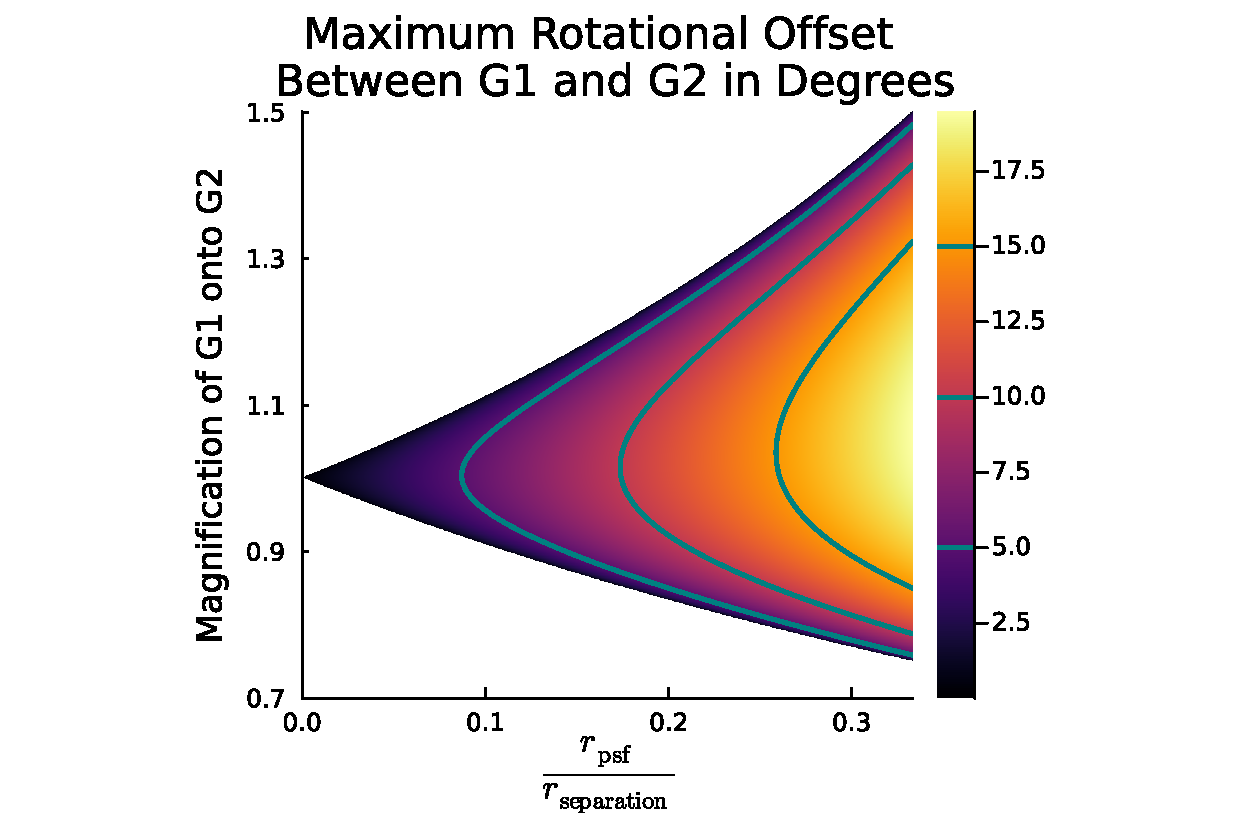
\includegraphics[width=0.6\textwidth]{figures/misalignments.pdf}
    \caption{Maximum rotational misalignment between G1 and G2 as a 
    function of G1 magnification and $\rho$.}
    \label{fig:Misalignments}
\end{figure}

Figure~\ref{fig:Misalignments} shows the maximum rotational misalignment $\theta$ before 
the diffraction spots appear like those created by a square grating (i.e. additional modes 
emerge). To get good qualtiy data, we'd likely want $\theta \leq \theta_\text{max}/2$.

I estimate Amy Turner's data of 2GMZI is within the $\rho \geq 0.2$ regime, permitting a maximum rotational offset 
of $10^\circ - 18^\circ$. Figure~\ref{fig:Misalignments_visuals} and \ref{fig:Misalignments_visuals_multiprobe} 
shows the diffraction spots for varying $\theta$ and $M$ at $\rho=0.3$. Figure Figure~\ref{fig:Misalignments_visuals} 
is for two-probes selected from G1 (0th and 1st order), while Figure~\ref{fig:Misalignments_visuals_multiprobe} is 
for all probes of G1. 

\begin{figure}[H]
    \centering
    \includegraphics[width=0.8\textwidth]{figures/rotational_effects_mags.pdf}
    \caption{Diffraction spots for varying rotational misalignment $\theta$ and magnification $M$. 
    $\rho=0.3$ was set, and both gratings (G1 and G2) are sinusoidal with mill depths 
    15.2nm and 23.2nm at 80keV. Two modes, the 0th and 1st order, of G1 are selected, i.e. the other 
    modes were removed. The predicted maximum rotational misalignment for each column is 
    $\theta_\text{max} = 8.96^\circ, 17.54^\circ, 16.09^\circ, 7.24^\circ$ for $M=0.8,1.0,1.2,1.4$, respectively.
    }
    \label{fig:Misalignments_visuals}
\end{figure}


\begin{figure}[H]
    \centering
    \includegraphics[width=0.8\textwidth]{figures/rotational_effects_mags_multiprobe.pdf}
    \caption{Diffraction spots for varying rotational misalignment $\theta$ and magnification $M$. 
    $\rho=0.3$ was set, and both gratings (G1 and G2) are sinusoidal with mill depths 
    15.2nm and 23.2nm at 80keV. All modes of G1 are selected were permitted. The predicted maximum 
    rotational misalignment for each column is 
    $\theta_\text{max} = 5.68^\circ, 8.75^\circ, 7.34^\circ, 0^\circ$ for $M=0.9,1.0,1.1,1.2$, respectively. 
    The effective $\rho$ was halved from the two-probe case because the distance from the -1st order to the 1st order 
    is doubled compared to the distance from the 0th order to the 1st order.
    }
    \label{fig:Misalignments_visuals_multiprobe}
\end{figure}

% \begin{figure}[H]
%     \centering
%     \begin{subfigure}{0.49\textwidth}
%         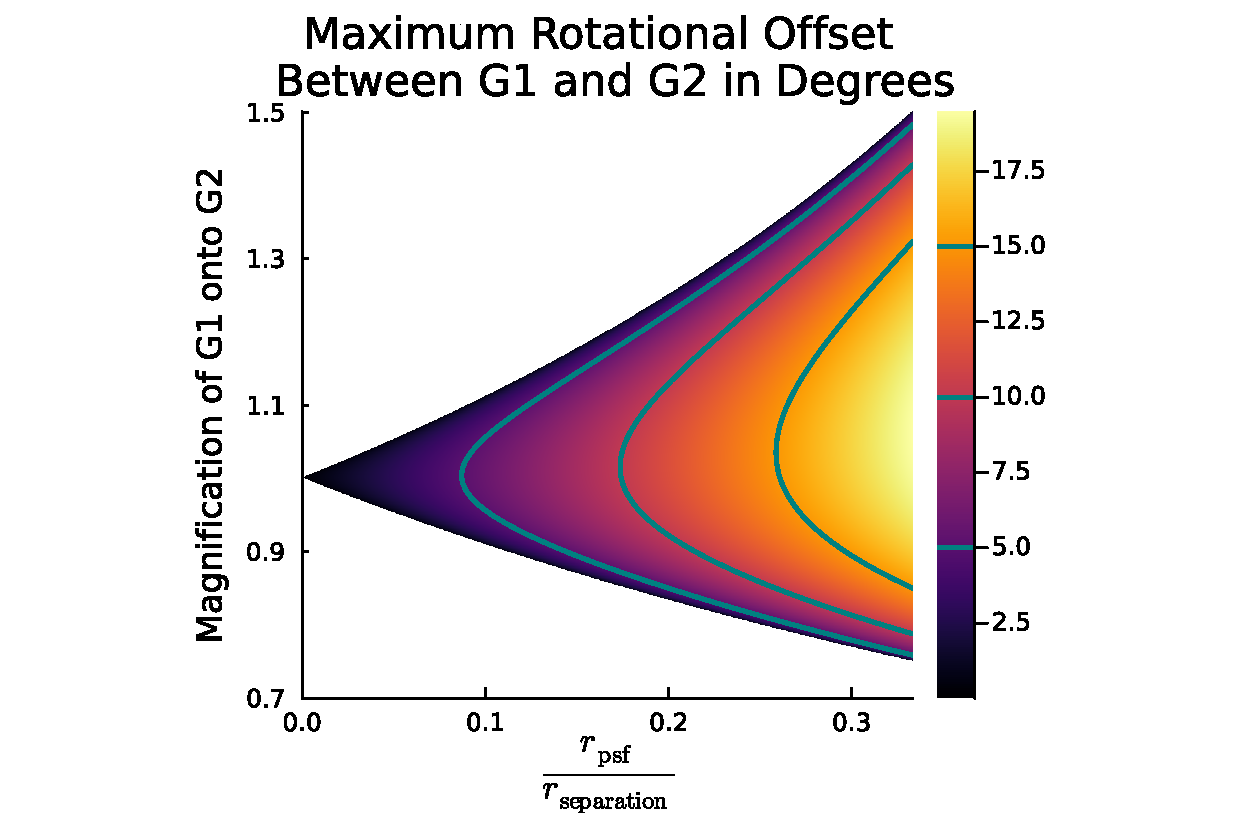
\includegraphics[width=\textwidth]{figures/misalignments.pdf}
%         \caption{Firts subfigure.}  
%         \label{fig:first}
%     \end{subfigure}
%     \hfill
%     \begin{subfigure}{0.49\textwidth}
%         \includegraphics[width=\textwidth]{figures/rotational_effects_mags.pdf}
%         \caption{Second subfigure.}
%         \label{fig:second}
%     \end{subfigure}
% \end{figure}


\section{Fourier (Transform, Series, and Coefficients)}
\subsection{Fourier Transform}
\begin{align}
    \FT{f(x)}(\xi) &= F(\xi)  = \int_{-\infty}^{\infty} f(x) e^{-i 2\pi \xi x} dx\\
    \FTinverse{F(\xi)}(x) &= f(x) = \int_{-\infty}^{\infty} F(k) e^{i 2\pi \xi x} d\xi
\end{align}
where $\xi = 1/d$ 
\subsection{Fourier Series}
A periodic function $f(x)$ with period $P$ can be represented as a unique sum of
complex exponentials:
\begin{equation}
    f(x) = \sum_{n=-\infty}^{\infty} c_n e^{i \frac{2\pi n}{P} x}
\end{equation}
where the Fourier coefficients $c_n$ are given by
\subsection{Fourier Coefficients}
\begin{equation}
    c_n = \frac{1}{P} \int_{0}^{P} f(x) e^{-i \frac{2\pi n}{P} x} dx
\end{equation}

\subsection{Connection}
The connection between the Fourier Transform and the Fourier coefficients can be seen with
the Fourier Transform of a periodic function with period P:
\begin{equation*}
    \FT{f(x)}(\xi) = \sum_{-\infty}^{\infty} c_n \cdot \delta(\xi - \frac{n}{P})
\end{equation*}

\section{Fourier Coefficients of Gratings}
Consider 1D phase diffraction gratings with period $p$, height $h$, and mill depth $d$. The 
height profile of these gratings can be represented by $g(x)$, and the transmission function is
\begin{equation}
    t(x) = e^{i \theta g(x)}
\end{equation}
where $\theta = \sigma V_{mip} + i \gamma$ determining the phase imparted; $\sigma$ is the interaction parameter, 
$V_{mip}$ is the mean inner potential, and $\gamma$ is the attenuation coefficient.
\subsection{Blazed}
\begin{equation}
    g_{bl}(x) = \frac{d}{p}x + (h-d) \quad 0 \leq x < P
\end{equation}
\begin{align*}
    c_n^{bl} &= \frac{1}{p} \int_{0}^{p} dx \,
        e^{i \theta (\frac{d}{p}x + (h-d))} e^{-i \frac{2\pi n}{p} x} \\
    &= \frac{e^{i \theta (h-d)}}{p} \int_{0}^{p} dx \, 
        e^{-i \frac{2\pi}{p} (n - \frac{\theta d}{2\pi}) x} \\
    &= \frac{e^{i \theta (h-d)}}{p}
        \frac{e^{-i \frac{2\pi}{p} (n - \frac{\theta d}{2\pi}) x}}{-i \frac{2\pi}{p} (n - \frac{\theta d}{2\pi})} \Big|_{0}^{p} \\
    &= \frac{e^{i \theta (h-d)}}{p} \frac{1}{-i \frac{2\pi}{p} (n - \frac{\theta d}{2\pi})}         
        \big(e^{-i 2\pi (n - \frac{\theta d}{2\pi})} - 1\big) \\
    &= \frac{e^{i \theta (h-d)}}{p} \frac{e^{-i \pi (n - \frac{\theta d}{2\pi})}}{-i \frac{2\pi}{p} (n - \frac{\theta d}{2\pi})} 
        \big(e^{-i \pi (n - \frac{\theta d}{2\pi})} - e^{i \pi (n - \frac{\theta d}{2\pi})}\big) \\
    &= \frac{e^{i \theta (h-d)}}{p} \frac{e^{-i \pi (n - \frac{\theta d}{2\pi})}}{-i \frac{2\pi}{p} (n - \frac{\theta d}{2\pi})} 
        \left(-2i \sin(\pi \qty(n - \frac{\theta d}{2\pi}))\right) \\
    &= e^{i \theta (h-d)} e^{-i \pi (n - \frac{\theta d}{2\pi})}
        \frac{\sin(\pi \qty(n - \frac{\theta d}{2\pi}))}{\pi \qty(n - \frac{\theta d}{2\pi})} \\
\end{align*}
\begin{equation}
    \boxed{c_n^{bl} = e^{i \theta (h-d)} \, 
    \sinc\qty(n - \frac{\theta d}{2\pi}) \,
    e^{-i \pi (n - \frac{\theta d}{2\pi})}}
\end{equation}


\begin{figure}[H]
    \centering
    % discrete |c_n| for several shifts a
    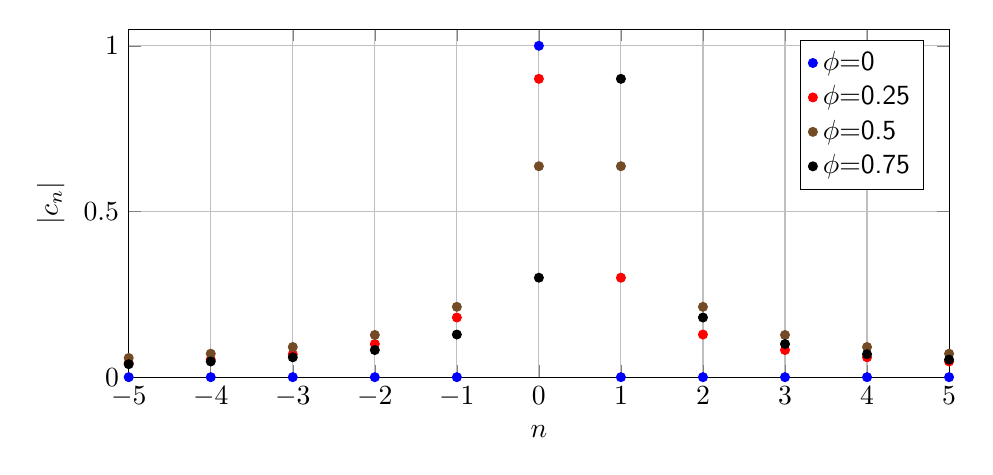
\begin{tikzpicture}
    \begin{axis}[
        xlabel={$n$},
        ylabel={$\abs{c_n}$},
        xmin=-5, xmax=5,
        ymin=0, ymax=1.05,
        xtick={-5,-4,...,5},
        grid=both,
        width=12cm, height=6cm,
        legend pos=north east,
        legend cell align=left,
        % cycle list name=exotic, % or leave default; we'll override color anyway
    ]
        % list the shifts you want to plot here
        \foreach \aval in {0,0.25, 0.5, 0.75}{
            \addplot+[
                only marks,
                mark=*,
                mark options={scale=0.8},
                samples=11,
                domain=-5:5
            ]
            % pgfplots math: abs() and ternary ?:
            {abs( (abs(x-\aval) < 1e-6) ? 1 : sin(deg(pi*(x-\aval))) / (pi*(x-\aval)) )};
            % legend text as plain text; pgfplots wraps it in math mode for us
            \addlegendentryexpanded{$\phi$=\aval}
        }
    \end{axis}
    \end{tikzpicture}
    \caption{Discrete amplitudes $\lvert c_n\rvert$ for a blazed grating for several fractional shifts $\phi=\frac{\Re(\theta)d}{2\pi}$.}
\end{figure}
\begin{align}
    c_n &= a e^{i\theta (h-d)} e^{-i \pi a (n-\beta_1)} \sinc(a(n - \beta_1)) \\
    &+ (1-a) e^{i\theta h} e^{-i n 2\pi a} e^{-i \pi (1-a)(n+\beta_2)} \sinc((1-a)(n + \beta_2))
\end{align}
where $\beta_1 = \frac{\theta d}{2\pi a}$ and $\beta_2 = \frac{\theta d}{2\pi (1-a)}$.
\begin{equation}
    c_n = a \frac{(\beta_1 + \beta_2)}{n+\beta_2} e^{i\theta (h-d)} e^{-i\pi a (n-\beta_1)} \sinc(a(n-\beta_1))
\end{equation}

\begin{equation}
    \sum_{n=0}^\infty |c_n|^2 = 1 \qquad \sum_{n=-\infty}^\infty |c_n|^2 = A
\end{equation}
% \printbibliography 
\end{document}